% -*- coding: utf-8; -*-
% vim: set fileencoding=utf-8 :
\documentclass[english,submission]{programming}
%% First parameter: the language is 'english'.
%% Second parameter: use 'submission' for initial submission, remove it for camera-ready (see 5.1)

\usepackage{longtable,booktabs}
% Correct order of tables after \paragraph or \subparagraph
\usepackage{etoolbox}
\makeatletter
\patchcmd\longtable{\par}{\if@noskipsec\mbox{}\fi\par}{}{}
\makeatother
% Allow footnotes in longtable head/foot
\IfFileExists{footnotehyper.sty}{\usepackage{footnotehyper}}{\usepackage{footnote}}
\makesavenoteenv{longtable}

\usepackage[backend=biber]{biblatex}
\addbibresource{references.bib}

\providecommand{\tightlist}{%
  \setlength{\itemsep}{0pt}\setlength{\parskip}{0pt}}

\begin{document}

\title{Wildcard: End user modification of web applications through a
data table}
\subtitle{}% optional

\author{Geoffrey Litt}
\authorinfo{is bla bla bla}
\author{Daniel Jackson}
\authorinfo{is bla bla bla}
\affiliation{Massachusetts Institute of Technology}

\keywords{programming journal, paper formatting, submission preparation} % please provide 1--5 keywords


%%%%%%%%%%%%%%%%%%
%% These data MUST be filled for your submission. (see 5.3)
\paperdetails{
  %% perspective options are: art, sciencetheoretical, scienceempirical, engineering.
  %% Choose exactly the one that best describes this work. (see 2.1)
  perspective=art,
  %% State one or more areas, separated by a comma. (see 2.2)
  %% Please see list of areas in http://programming-journal.org/cfp/
  %% The list is open-ended, so use other areas if yours is/are not listed.
  area={Social Coding, General-purpose programming},
  %% You may choose the license for your paper (see 3.)
  %% License options include: cc-by (default), cc-by-nc
  % license=cc-by,
}
%%%%%%%%%%%%%%%%%%

%%%%%%%%%%%%%%%%%%
%% These data are provided by the editors. May be left out on submission.
%\paperdetails{
%  submitted=2016-08-10,
%  published=2016-10-11,
%  year=2016,
%  volume=1,
%  issue=1,
%  articlenumber=1,
%}
%%%%%%%%%%%%%%%%%%

%%%%%%%%%%%%%%%%%%%%%%%%%%%%%
% Please go to https://dl.acm.org/ccs/ccs.cfm and generate your Classification
% System [view CCS TeX Code] stanz and copy _all of it_ to this place.
%% From HERE
\begin{CCSXML}
<ccs2012>
<concept>
<concept_id>10002944.10011122.10003459</concept_id>
<concept_desc>General and reference~Computing standards, RFCs and guidelines</concept_desc>
<concept_significance>300</concept_significance>
</concept>
<concept>
<concept_id>10010405.10010476.10010477</concept_id>
<concept_desc>Applied computing~Publishing</concept_desc>
<concept_significance>300</concept_significance>
</concept>
</ccs2012>
\end{CCSXML}

\ccsdesc[300]{General and reference~Computing standards, RFCs and guidelines}
\ccsdesc[500]{Applied computing~Publishing}

% To HERE
%%%%%%%%%%%%%%%%%%%%%%%

\maketitle

% Please always include the abstract.
% The abstract MUST be written according to the directives stated in 
% http://programming-journal.org/submission/
% Failure to adhere to the abstract directives may result in the paper
% being returned to the authors.
\begin{abstract}
Browser extensions and user scripts can modify web applications in
useful ways, but many people have unique needs that aren't met by
existing extensions. Today, most of those people can't build their own
browser extensions, since they can't program in Javascript.

Wildcard is a platform that empowers anyone to build browser extensions
without doing traditional programming. Wildcard shows the main data from
a web page in a table that maintains a bidirectional connection to the
original page. By directly manipulating the table, people can
sort/filter content, add private annotations, and use spreadsheet
formulas to fetch data from other websites.
\end{abstract}


\hypertarget{introduction}{%
\section{Introduction}\label{introduction}}

In 2012, the travel site Airbnb removed the ability to sort listings by
price. Users could still filter down to a price range, but could no
longer view the cheapest listings first. Many users complained on online
message boards that the change seemed hostile to users. ``It's so
frustrating!..What is the logic behind not having this function?'' says
one user on the
\href{https://community.withairbnb.com/t5/Hosting/Sorting-listing-by-price/td-p/559404}{Airbnb
support forum}. Alas, the feature remains missing to this day.

This is a familiar situation in a world of web applications that are
frequently updated without user consent. When web software doesn't quite
meet users' needs, their only recourse is to complain to the developers
and hope someone listens. Sometimes there is a way to use a browser
extension or user script to fix the issue, but making an extension
requires sophisticated programming skills. We see this as a waste of the
openness of the Web platform, and of the pliability of software in
general. If users could make tweaks to web applications without
programming, a vast number of people would gain the agency to modify
software to meet their unique preferences.

In this paper, we introduce a system called Wildcard\footnote{Wildcard
  was the original internal name for Hypercard, which pioneered both
  user modifiable software and the modern Web.} that aims to meet this
need. Wildcard adds a panel to the bottom of a web page that shows a
structured table view of some of the main data in the page. The table
maintains a bidirectional connection to the original page---when the
user manipulates the table, the original page also gets modified, and
vice versa.

In Wildcard, sorting Airbnb listings by price takes just one click on a
table header, with no programming required by the end user. Beyond
sorting and filtering data, Wildcard also supports a variety of other
use cases like accessing third party APIs, performing small
computations, recording private user annotations, and using alternate UI
widgets. While Wildcard does not support all changes someone might want
to make to a website, the goal of the project is to make a broad subset
of changes easily accessible to end users.

Under the hood, there is no magic---Wildcard currently requires a
programmer to manually define an adapter between the original page and
the data table using web scraping techniques. While programming is
required for part of the process, this forms a useful collaboration
between the programmer and the end user, since the end user is able to
perform many different modifications once an adapter is defined. We also
plan to eventually reduce the burden of making adapters (discussed in
more detail later).

\hypertarget{demo-booking-a-trip-with-wildcard}{%
\section{Demo: Booking a trip with
Wildcard}\label{demo-booking-a-trip-with-wildcard}}

To get a sense of the user experience of Wildcard, let's see an example
of how an end user can modify a website with Wildcard in practice.

For example, in Fig.~\ref{fig:table} we open up a table view that
corresponds to search results on the Airbnb travel site.

\begin{figure}
\hypertarget{fig:table}{%
\centering
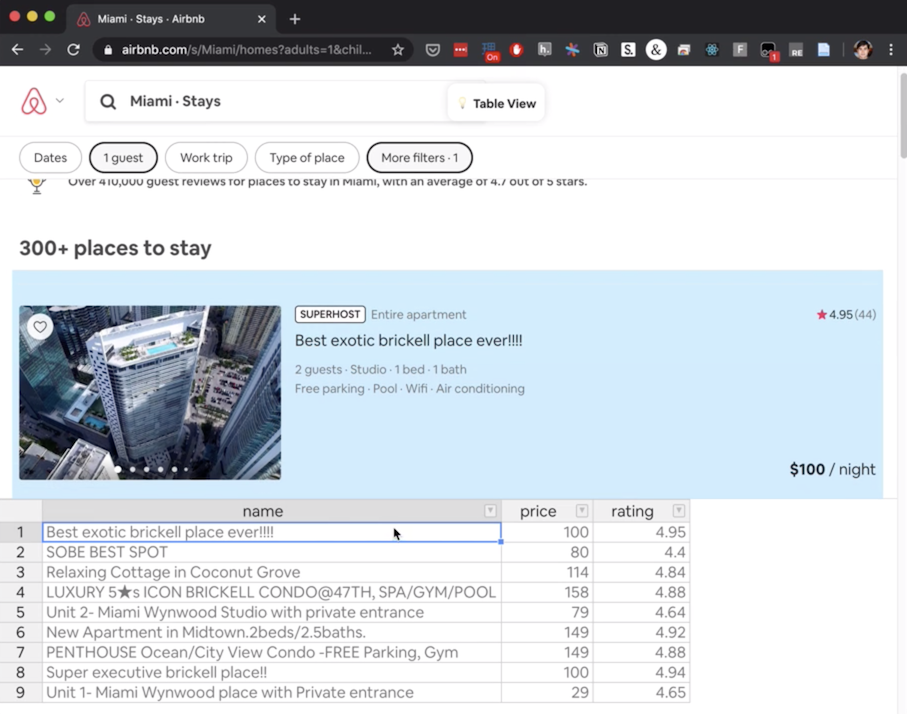
\includegraphics{media/opentable.png}
\caption{Opening a table corresponding to search results on
Airbnb}\label{fig:table}
}
\end{figure}

\begin{itemize}
\tightlist
\item
  Sorting search results:

  \begin{itemize}
  \tightlist
  \item
    Airbnb took away search
  \item
    once you see the tabular view, there's an obvious interaction
    available to anyone familiar with tables
  \end{itemize}
\item
  Injecting new data into the page

  \begin{itemize}
  \tightlist
  \item
    Take own custom notes, saved in the browser. Maybe shared in the
    future
  \end{itemize}
\item
  Formulas

  \begin{itemize}
  \tightlist
  \item
    Compute values to inject into the page
  \item
    TBD: styling
  \end{itemize}
\item
  Using a custom date picker
\end{itemize}

\hypertarget{system-implementation}{%
\section{System Implementation}\label{system-implementation}}

\emph{Goal of this section: briefly explain the current implementation.
Enough detail to ground further discussion, but don't dwell on it. It's
not the main point, and will evolve a lot.}

\begin{itemize}
\tightlist
\item
  Built as a Greasemonkey script for now (\emph{todo: convert to a full
  broser extension?})
\item
  Describe the adapter API

  \begin{itemize}
  \tightlist
  \item
    programmer creates adapters for now
  \item
    maybe end users can create in the future, or automated
  \item
    show a snippet of adapter code
  \end{itemize}
\item
  Mention the technique of scraping data from AJAX requests
\item
  future implementation goals

  \begin{itemize}
  \tightlist
  \item
    make it easy for programmers to add adapters + plugins, and
    distribute them to users. (Currently all adapters + plugins are part
    of the main Wildcard codebase)
  \end{itemize}
\end{itemize}

\hypertarget{design-principles}{%
\section{Design principles}\label{design-principles}}

Below are some of the ideas behind the design of Wildcard. We hope that
these principles are also useful for thinking more broadly about
enabling end users to modify software.

\hypertarget{expose-unified-structure-across-applications}{%
\subsection{Expose unified structure across
applications}\label{expose-unified-structure-across-applications}}

\emph{Todo: add a diagram here?}

In \emph{Changing Minds} \autocite{disessa2000}, Andrea diSessa
critiques the design of modern software with a story about a
hypothetical ``nightmare bike.'' Each gear on the nightmare bike is
labeled not with a number, but with an icon describing its intended use:
smooth pavement uphill, smooth pavement downhill, gravel, etc. By some
logic, this is more ``user-friendly'' than numbered gears, but in fact,
hiding orderly structure from the user makes it more difficult to
operate the bike. Many modern software designs fall into this trap,
teaching users to use isolated modes rather than coherent structure, and
the problem gets far worse when operating across multiple applications.
Unlike the UNIX philosophy of small tools interoperating through shared
abstractions, in modern computing each application is in its own silo of
data and functionality.

Wildcard helps people understand and modify the behavior of applications
through the lens of a consistent abstraction: a data table. This
abstraction strikes a balance between being both simple and generic. A
data table is simpler than the DOM tree that describes the details of
the UI, but is also generic enough to describe the essence of many
different kinds of applications.

Exposing a unified higher-level abstraction is a deliberate choice, and
is not the only way to enable users to program without directly using
the DOM. Chickenfoot \autocite{bolin2005} and CoScripter
\autocite{leshed2008} allow users to create scripts that resemble
natural language and ``sloppily'' match queries to elements in the DOM.
These designs allow for a wide range of operations, but don't explicitly
indicate what operations are possible---the user must look at the
original page and imagine the possibilities. In contrast, Wildcard
provides affordances that clearly suggest the availability of certain
types of modifications. In addition to giving users more certainty about
whether a modification is possible, these affordances might give users
new ideas for things to try. Because people are not used to modifying
web applications, providing inspiration is an important goal. (Todo:
Perhaps something to cite here, re: discoverability in GUIs vs CLIs?)

\hypertarget{direct-manipulation-by-proxy}{%
\subsection{Direct manipulation by
proxy}\label{direct-manipulation-by-proxy}}

In Wildcard, users manipulate a data table added to the page, rather
than the original page. Although the interaction with the table is
direct like using a spreadsheet, the interaction with the page is
indirectly mediated through the table.

We considered other approaches where the user would interact more
directly with the original UI, e.g.~injecting sort controls into the
page, but decided that the consistency and affordances of the table view
outweighed the potential confusion of a new layer of indirection.

Making this design successful requires maintaining a close mapping in
the user's mind between the new representation and the original page
(cite Norman? Cognitive Dimensions?). Wildcard provides live visual cues
as the user navigates the data table, similar to the highlighting
provided by browser developer tools to indicate the mapping between HTML
and the original page.

\begin{figure}
\hypertarget{fig:devtools}{%
\centering
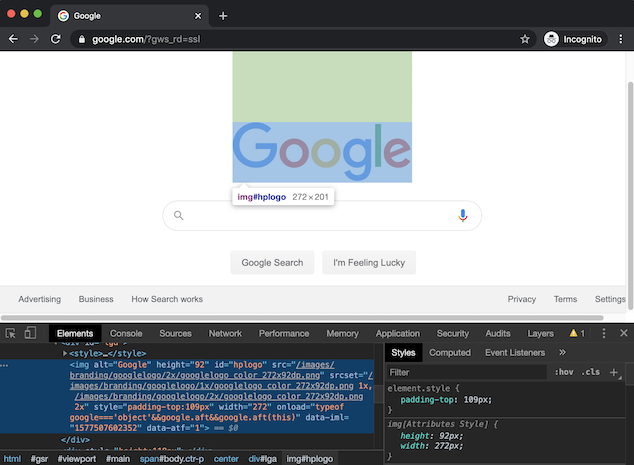
\includegraphics{media/devtools.png}
\caption{The Chrome Dev Tools use highlighting to show the mapping
between HTML code and the page}\label{fig:devtools}
}
\end{figure}

\hypertarget{decouple-ui-from-data}{%
\subsection{Decouple UI from data}\label{decouple-ui-from-data}}

Most software does not provide much user choice for interface elements,
even for common data types: e.g., the website provides a datepicker
widget, and you have no ability to provide your own replacement
datepicker. This forces users to learn many different interfaces for
similar tasks, some of them worse than others. It also prevents
combining data across multiple applications within a single user
interface.

Wildcard exposes the data underlying an application's UI, allowing the
user to use interfaces of their choice to view and modify the data. The
Expedia datepicker demo above showed one example of how this can be
useful, but we also envision creating other widgets for visualizing and
editing data. Some examples would be showing geographic data in a custom
map that includes the user's own annotations, or editing a blog post in
a rich text editor of the user's choice.

One benefit of decoupling data from interfaces is improved UI quality.
When UI widgets can compete on their merits rather than based on network
effects from the data they have access to, it creates much stronger
competition at the interface level. For example, there is competition
among email clients (which consume an open protocol), but not among
Facebook or Twitter clients. This benefit relates to the SOLID project
led by Tim Berners-Lee \autocite{berners-lee2018}, which envisions
user-controlled data as a mechanism for decoupling data from interfaces,
e.g.~giving users a choice of which client to use to consume a given
social media feed. Wildcard has overlapping goals with SOLID, but does
not require decentralized user control of data---the data can remain on
a centralized server, as long as the interface can be tweaked by end
users. \emph{Note: maybe this paragraph belongs in related work?}

There is also value in using the same consistent interface across many
applications. For example, many programmers become deeply familiar with
one text editor and use it for many different kinds of tasks. This usage
even extends beyond editing permanent files; shell programs can use the
user's preferred text editor as an interactive input mechanism (e.g.~for
editing git commit messages). This ability to generically reuse the text
editor in many contexts makes it more worthwhile to invest time
mastering the tool. Beaudouin-Lafon and Mackay refer to this type of
reuse as \emph{polymorphism} in interaction
\autocite{beaudouin-lafon2000}, noting that it is a key technique for
keeping interfaces simple while increasing their power.

\emph{Note: Maybe could relate this section to Concept Reuse?}

\emph{Note: Does this section overlap with ``expose unified
structure''?}

\hypertarget{in-place-toolchain}{%
\subsection{In-place toolchain}\label{in-place-toolchain}}

\begin{longtable}[]{@{}lll@{}}
\toprule
\endhead
& \textbf{In-place} & \textbf{Not in-place}\tabularnewline
\textbf{End user friendly} & Wildcard & IFTTT\tabularnewline
\textbf{For developers} & browser dev tools & editing OSS\tabularnewline
\bottomrule
\end{longtable}

We believe that people are more motivated to modify software when the
tools for modification are close at hand while using the original
software, referred to by Ink and Switch as an ``in-place toolchain''
\autocite{inkandswitch2019}.

Browser developer tools exemplify an in-place toolchain, since they are
built in to browsers and available in the context of viewing a page; in
contrast, creating a browser extension requires moving out of the
browser to a separate development environment.

Wildcard creates an in-place toolchain for modifying web applications.
Once installed, if an adapter is available for a site, it can be
immediately modified from within the browser. Hopefully, this can help
make switching from using to modifying software into a smooth
transition, rather than a chasm to cross.

\hypertarget{first-party-cooperation-optional}{%
\subsection{First party cooperation
optional}\label{first-party-cooperation-optional}}

The Web is an unusually extensible platform. On many other platforms
(e.g.~smartphone operating systems), software is locked down unless
first-party developers explicitly provide hooks for plugins and
interoperability, but on the Web, all client-side code is available for
browser extensions to modify. Application authors can use practices that
make it easier to modify their apps (e.g.~clean semantic markup), or
more difficult (e.g.~code obfuscation), but the default state is
openness. This gives extensions freedom to modify applications in
creative ways that the original developers did not plan for.

Wildcard takes advantage of this openness, and does not depend on
cooperation from first-party website developers. Any programmer can add
support for any website to Wildcard by building a third party adapter.
This design acknowledges the pragmatic reality that most sites today
will not have Wildcard support built in, and more broadly do not
prioritize client side extensibility.

However, we also hope that first party website developers eventually
build in Wildcard support to their applications, which would reduce the
burden of maintaining adapters and make Wildcard plugins more stable.
While this might seem optimistic, implementing the Wildcard adapter API
could be straightforward in a typical client-side application that
already has access to a structured version of the data in the page.
There is also precedent for first parties implementing an official
client extension API in response to user demand: for several years,
Google exposed an extension API in Gmail for Greasemonkey scripts to
use. (Since then, third parties have created well-maintained
alternatives \autocite{streak,talwar2019}, illustrating the value of
sharing even third party adapters.)

\hypertarget{related-work}{%
\section{Related work}\label{related-work}}

\emph{Note: a lot of this was already covered above; how to deal with
that?}

\begin{itemize}
\tightlist
\item
  Instrumental interaction
\item
  Web automation
\item
  Wrapper induction
\item
  Personal data ownsership / SOLID
\item
  Extension helper libraries, e.g.~Gmail.js.
\end{itemize}

\hypertarget{future-work}{%
\section{Future work}\label{future-work}}

\begin{itemize}
\tightlist
\item
  still in early development; note the beta release plan (tentative:
  target public beta availability at the workshop in March?)
\item
  What are the limits of functionality? What can't it do?

  \begin{itemize}
  \tightlist
  \item
    Should we extend further? Automation workflows? Triggers?
  \end{itemize}
\item
  Could explore automated wrapper induction, building on prior work
\item
  Usability studies
\item
  Link to sign up for future updates
\end{itemize}

\acks
\printbibliography

\end{document}

% Local Variables:
% TeX-engine: luatex
% End:
